\documentclass[10pt]{article}
\usepackage[spanish]{babel}
\usepackage[utf8]{inputenc}
\usepackage[T1]{fontenc}
\usepackage[margin=1.2cm, footskip=0.45cm]{geometry}
\usepackage{graphicx}
\usepackage{amsmath}
\usepackage{booktabs}
\usepackage{float}
\usepackage{tabularx}
\usepackage{caption}
\usepackage{subcaption}
\usepackage{hyperref}

\hypersetup{colorlinks=true, linkcolor=black, urlcolor=blue, citecolor=black}
\setlength{\parindent}{0pt}
\setlength{\parskip}{0.22em}
\setlength{\tabcolsep}{4pt}
\renewcommand{\arraystretch}{1.05}
\captionsetup{font=small, labelfont=bf}

\title{\textbf{Proyecto 2 - Freesound Audio Tagging}\\Taller de Aprendizaje Automático}
\author{Luciana García \and Santiago Márquez \and Santiago Rodríguez}
\date{\today}

\begin{document}
\maketitle

\section{Introducción}
El problema consiste en asignar etiquetas sonoras a audios de Freesound. Es una
tarea \textit{multi-label}: una grabación puede contener varias fuentes de sonido
y la salida debe ser una probabilidad para cada una de las 80 clases. La métrica
usada por Kaggle es \textit{label-weighted label-ranking average precision}
(lwlrap), que premia que las etiquetas correctas queden bien rankeadas para
cada audio.

La primera entrega consolidada usaba un ensamble de tres ramas entrenadas 100
épocas sobre \texttt{train\_curated}. Ese sistema obtuvo \textbf{0.67126} en el
private leaderboard de Freesound Audio Tagging 2019. La versión final de este
informe toma ese modelo como punto de partida y agrega una segunda etapa:
continuar el entrenamiento con datos curados y ruidosos, pero controlando el
impacto de \texttt{train\_noisy}. El resultado final fue \textbf{0.68122} en el
private leaderboard de Freesound 2019 y \textbf{0.64307} en el leaderboard
público del Kaggle del curso.

\section{Datos y métrica}
El dataset contiene tres fuentes principales: \texttt{train\_curated.csv},
\texttt{train\_noisy.csv} y \texttt{sample\_submission.csv}. El conjunto curado
es pequeño pero confiable; el conjunto ruidoso tiene más ejemplos, aunque sus
etiquetas son menos seguras. Esa diferencia motivó no concatenar ambos conjuntos
sin control.

\begin{table}[H]
\centering
\small
\begin{tabular}{@{}lrrr@{}}
\toprule
Split & Filas & Rol & Uso final \\
\midrule
train\_curated & 4970 & etiquetas confiables & base y 50\% de cada batch \\
train\_noisy & 19815 & mayor cobertura, etiquetas ruidosas & 50\% de cada batch, peso 0.30 \\
test & 3361 & audios a predecir & submission final \\
\bottomrule
\end{tabular}
\caption{Conjuntos usados. El fine-tuning usa noisy con menor peso para aportar
variabilidad sin dominar la señal curada.}
\end{table}

\begin{figure}[H]
\centering
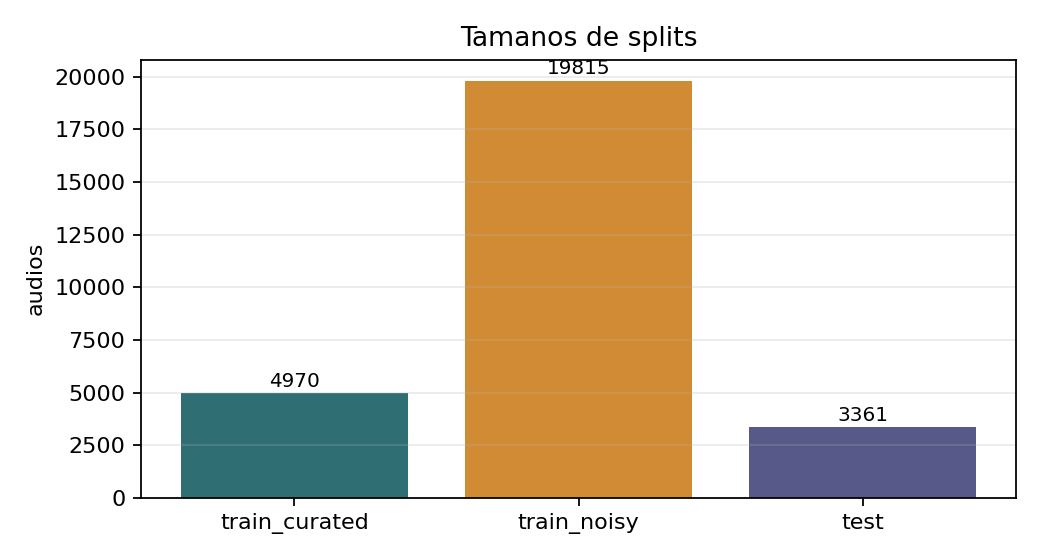
\includegraphics[width=0.62\textwidth]{img/fig_v2_split_sizes.png}
\caption{Tamaño relativo de los tres splits.}
\end{figure}

La métrica lwlrap se puede leer como un promedio ponderado de precisión en
ranking. Para cada audio se ordenan las clases por probabilidad y se mira si las
clases verdaderas aparecen arriba:
\[
\mathrm{lwlrap}=\sum_{c=1}^{C}w_c\frac{1}{N_c}\sum_{i:y_{ic}=1}
\mathrm{precision}_{i,c}.
\]
Por esto el promedio de modelos es natural: ramas con errores distintos pueden
mejorar el ranking final aunque cada una no sea perfecta.

\section{Representación de audio}
Cada archivo \texttt{.wav} se convierte en una imagen log-mel:
\begin{center}
\texttt{.wav -> mono -> 44.1 kHz -> MelSpectrogram -> log/dB -> crop/pad -> normalización}
\end{center}
Se usan 128 bandas Mel. El eje horizontal representa tiempo y el eje vertical
frecuencia perceptual. Las ramas principales usan entradas \texttt{128 x 512};
la rama temporal larga usa \texttt{128 x 1024}.

\begin{figure}[H]
\centering
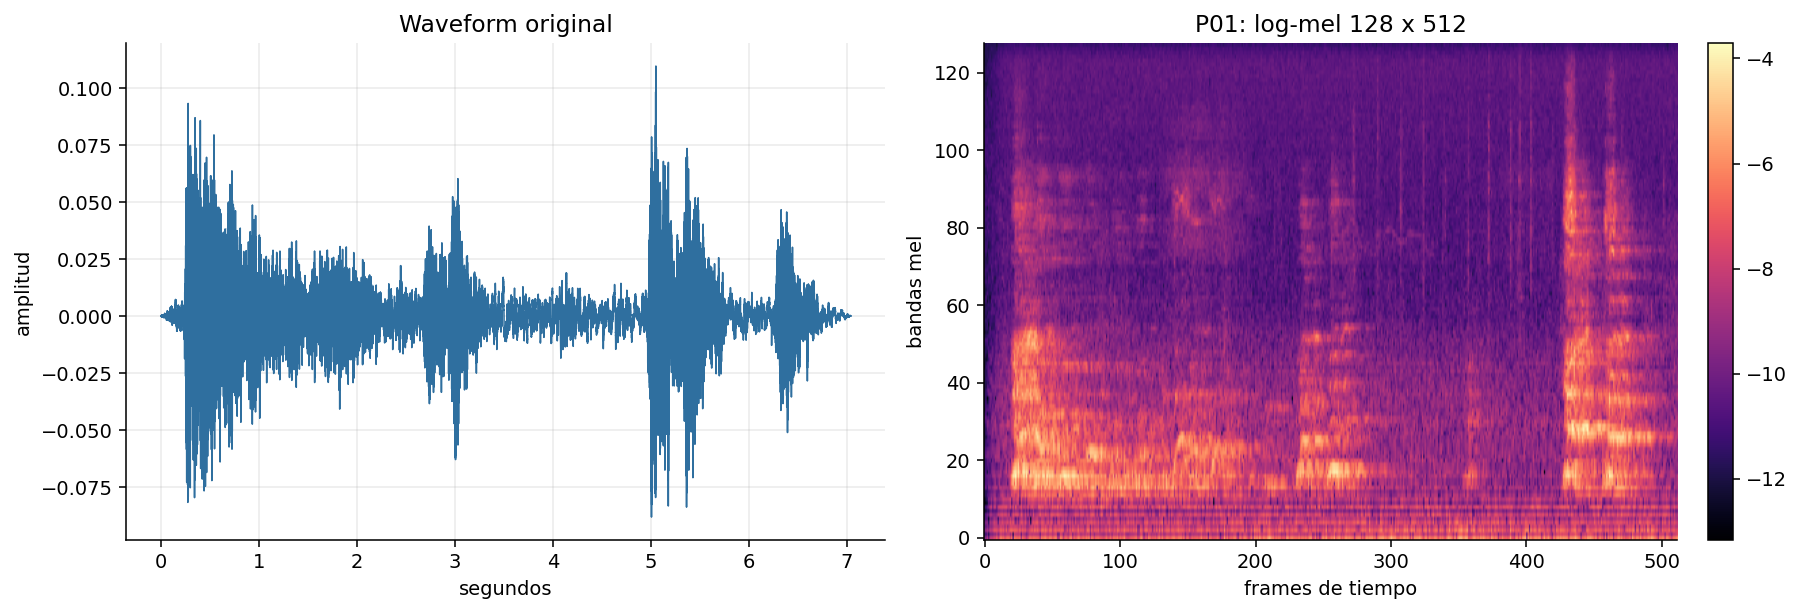
\includegraphics[width=0.78\textwidth]{img/fig_waveform_logmel.png}
\caption{Pasaje de forma de onda a imagen log-mel. La red aprende patrones
tiempo-frecuencia sobre esta representación.}
\end{figure}

\section{Modelo base: ensamble 3-way e100}
Antes del experimento final se fijó un ensamble defendible de tres ramas:
\begin{itemize}
\item \textbf{H100}: CNN separable-residual con cabeza densa, log-mel
\texttt{128 x 512}, normalización por clip.
\item \textbf{G100}: CNN separable con cabeza temporal BiGRU y normalización
global por banda Mel.
\item \textbf{F100}: misma familia temporal, pero con ventana
\texttt{128 x 1024} para conservar más contexto.
\end{itemize}

La combinación usada fue:
\[
0.25\,H100 + 0.375\,G100 + 0.375\,F100.
\]
Este sistema obtuvo \textbf{0.67126}. También se habían probado variantes más
complejas, por ejemplo bagging, con score \textbf{0.67674}; sin embargo, esa
mejora era menos limpia conceptualmente. El experimento final buscó una mejora
manteniendo la misma arquitectura de tres caminos.

\begin{figure}[H]
\centering

\includegraphics[width=0.48\textwidth]{img/fig_v2_component_weights.png}
\caption{Pesos del ensamble final. Se conservaron los mismos pesos que en el
modelo 3-way e100.}
\end{figure}

\section{Experimento final: noisy fine-tune}
\subsection{Hipótesis}
La hipótesis fue que el modelo e100 ya había aprendido una representación fuerte
desde etiquetas curadas, pero aún podía beneficiarse de la variedad de
\texttt{train\_noisy} si la segunda etapa era conservadora. Por eso se aplicaron
cuatro restricciones:
\begin{enumerate}
\item partir de los checkpoints finales del ensamble 3-way;
\item usar learning rate bajo, \texttt{1e-4}, con scheduler coseno;
\item formar batches mitad \texttt{curated} y mitad \texttt{noisy};
\item pesar las filas noisy con 0.30 en la pérdida.
\end{enumerate}
Además se usó data augmentation online sobre log-mel: time shift, time mask,
frequency mask y ruido gaussiano.

\subsection{Configuración}
\begin{table}[H]
\centering
\small
\begin{tabularx}{\textwidth}{@{}lrrX@{}}
\toprule
Rama & Frames & Peso ensamble & Segunda etapa \\
\midrule
separable\_headsep & 512 & 0.250 & 30 épocas, batches 50/50, noisy 0.30 \\
globalmel\_sep\_temporal & 512 & 0.375 & 30 épocas, global-mel, noisy 0.30 \\
sep\_temporal\_f1024 & 1024 & 0.375 & 30 épocas, memmap para evitar OOM, noisy 0.30 \\
\bottomrule
\end{tabularx}
\caption{Configuración de la continuación final.}
\end{table}

\begin{figure}[H]
\centering

\includegraphics[width=0.70\textwidth]{img/fig_v2_branch_local.png}
\caption{Control local de degradación. La validación local no es independiente:
los checkpoints base fueron entrenados con todo curated.}
\end{figure}

La Figura anterior no se interpreta como estimación real del leaderboard, porque
los modelos base ya habían visto todo \texttt{train\_curated}. Sirve para
detectar degradaciones grandes; la decisión final se toma con Kaggle.

\section{Resultados}
\begin{figure}[H]
\centering

\includegraphics[width=0.80\textwidth]{img/fig_v2_kaggle_scores.png}
\caption{Scores relevantes. El Kaggle del curso usa una variante del dataset y
se reporta separado.}
\end{figure}

\begin{table}[H]
\centering
\small
\begin{tabular}{@{}lrr@{}}
\toprule
Referencia & Score & Lectura \\
\midrule
3-way e100 anterior & 0.67126 & punto final previo \\
Mejor variante previa registrada & 0.67674 & bagging, más compleja \\
Noisy fine-tune Freesound 2019 private & \textbf{0.68122} & nuevo mejor público del historial \\
Noisy fine-tune Kaggle del curso public & \textbf{0.64307} & referencia en variante de datos del curso \\
\bottomrule
\end{tabular}
\caption{Resultados principales.}
\end{table}

La mejora contra el punto final anterior es:
\[
0.68122 - 0.67126 = 0.00996.
\]
Contra la mejor variante previa registrada:
\[
0.68122 - 0.67674 = 0.00448.
\]
El CSV final tiene 3361 filas, 80 columnas de etiquetas, probabilidades en
\([0,1]\), mismo orden de \texttt{fname} que \texttt{sample\_submission.csv} y
hash SHA256:
\begin{center}
\small\texttt{b29288caa6e7b37b29e830a29655decc7c6bc8110ca3a40b828f4dd2f5fabdcc}
\end{center}

\section{Conclusión}
La contribución final no fue cambiar la arquitectura, sino cambiar el protocolo
de entrenamiento. Primero se aprende de etiquetas confiables durante 100 épocas;
luego se usa el conjunto ruidoso como regularizador y fuente de cobertura, pero
con batches balanceados, peso reducido y learning rate bajo. Esta estrategia
mantiene la claridad del ensamble de tres caminos y mejora el resultado de
leaderboard. Para la defensa, el mensaje central es que \texttt{train\_noisy}
no se descartó ni se incorporó ingenuamente: se incorporó con una política
explícita de confianza parcial.

\end{document}

